\documentclass[a4paper,12pt]{article}

\usepackage{times}
\usepackage[french]{babel}
\usepackage[utf8x]{inputenc}
\usepackage[T1]{fontenc}
\usepackage{amsmath}
\usepackage{amssymb}
\usepackage{graphicx}
\usepackage{pdfpages}
\usepackage{pdflscape}
\usepackage{listings}
\usepackage{longtable}
\setlength{\topmargin}{0cm}
\setlength{\headsep}{0.1in}
\setlength{\headheight}{10 pt}
\setlength{\evensidemargin}{0cm}
\setlength{\oddsidemargin}{-1cm}
\textwidth 18cm
\textheight 25cm


\usepackage{fancyhdr}
\pagestyle{fancy}
\fancyhf{}
\lhead{\scriptsize{\bsc{Projet Logiciel Transversal}}}
\rhead{\scriptsize{Les Dee \& Di}}
\renewcommand{\footrulewidth}{0.5pt}
\rfoot{\scriptsize{\bsc{Ayroles}, \bsc{El Bèze}, \bsc{Maerten}}}
\lfoot{\thepage}
\lstset{literate=
{é}{{\'e}}1
{è}{{\`e}}1
{ê}{{\^e}}1
{à}{{\`a}}1
{â}{{\^a}}1
}
\lstset{language=C++,
                basicstyle=\footnotesize,
                keywordstyle=\footnotesize\color{blue},
                otherkeywords={override,nullptr}
}
\definecolor{orange}{rgb}{0.8,0.4,0.0}
\definecolor{darkblue}{rgb}{0.0,0.0,0.6}
\definecolor{cyan}{rgb}{0.0,0.6,0.6}
\lstdefinelanguage{JSON}
{
  basicstyle=\normalsize,
  columns=fullflexible,
  showstringspaces=false,
  commentstyle=\color{gray}\upshape,
  morestring=[b]",
  morestring=[s]{>}{<},
  morecomment=[s]{<?}{?>},
  stringstyle=\color{orange},
  identifierstyle=\color{darkblue},
  keywordstyle=\color{blue},
  morekeywords={string,number,array,object}% list your attributes here
}


\sloppy



\begin{document}

\renewcommand{\labelitemi}{$\bullet$}

\thispagestyle{empty}

\title{\large Projet Logiciel Transversal\\[0.5cm]
        \bf\Large Les Dee \& Di}
\author{\large \bsc{Ayroles} Quentin, \bsc{El Bèze} Ilan, \bsc{Maerten} Eloïse}
\date{2021 - 2022}
\makeatletter
    \begin{titlepage}
        \begin{center}
        \vbox{}\vspace{5cm}
            {\@title }\\[3cm] 
            {\@author}\\
            %{Instructor: \bf instructor name}\\
%            \vfill \includegraphics[scale=0.3]{images/logo.png}\\[1cm]
            {\@date}
        \end{center}
    \end{titlepage}
\makeatother
%\thispagestyle{empty}


\clearpage

{\small
\tableofcontents
}



\clearpage
\section{Présentation Générale}

\subsection{Archétype}
L’objectif de ce projet est la réalisation d’un jeu de rôle (RPG) classique inspiré par Donjons \& Dragons.

\subsection{Règles du jeu}
Le but du joueur est de réaliser la quête définie en début de partie. Pour cela il dispose d'une équipe de 6 héros avec 6 rôles différents (Guerrier, Magicien, Assassin, Archer, Druide, Prêtre). Si le joueur est seul, il joue les 6 héros. En cas de multijoueur le joueur joue les classes qu'il choisit en début de partie (il y a donc au maximum 6 joueurs sur la même partie, si le nombre de joueurs est inférieur à 6, certains joueront plusieurs héros). Le multijoueur sera donc coopératif. Les joueurs évoluent sur une carte (sous forme de grille). Sur la carte, les joueurs peuvent être confrontés à des ennemis, événements et réaliser diverses actions(comme lancer des sorts). Ces actions auront une part d’aléatoire pour imiter les lancer de dés du jeu original. À terme, l’idée est d’aussi permettre au joueur de collecter des objets et d'améliorer ses personnages. 

\subsection{Ressources}

\begin{figure}[hbt!]
    \centering
    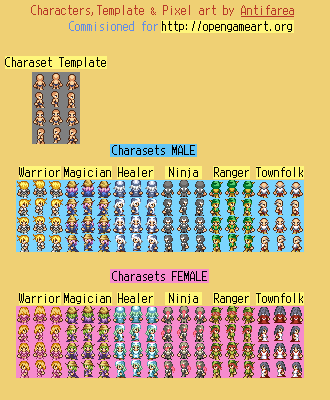
\includegraphics[scale=0.9, angle=0]{images/texture_persos1.png}
    \caption{Textures des personnages}
    \label{fig:textPerso}
\end{figure}

\begin{figure}[hbt!]
    \centering
    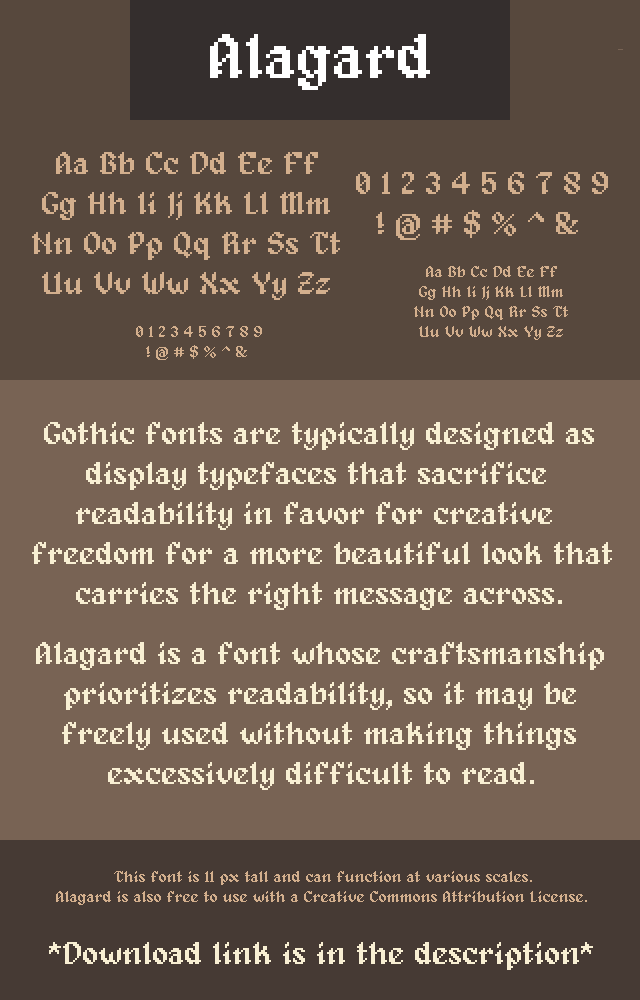
\includegraphics[scale=0.3, angle=0]{images/fonts.png}
    \caption{Police d'écriture}
    \label{fig:fonts}
\end{figure}

\begin{figure}[hbt!]
    \centering
    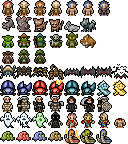
\includegraphics[scale=2, angle=0]{images/texture_monstres1.png}
    \caption{Textures des ennemies}
    \label{fig:textEnnemis}
\end{figure}

\begin{figure}[hbt!]
    \centering
    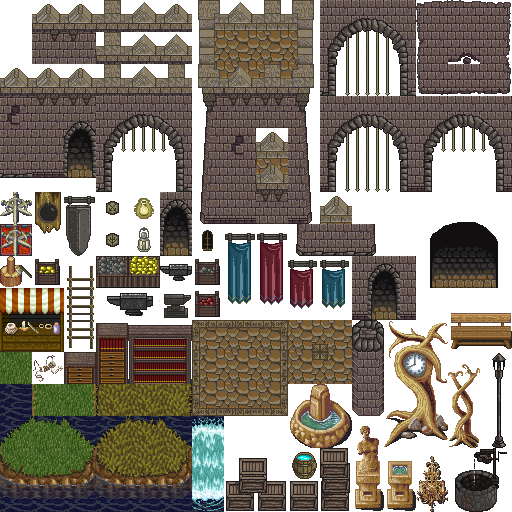
\includegraphics[scale=1.5, angle=0]{images/texture_decor1.png}
    \caption{Textures des décors}
    \label{fig:textDecor}
\end{figure}


\clearpage
\section{Description et conception des états}

\subsection{Description des états}
Un état de jeu est constitué d'un décor (tableaux d'éléments représentant la grille du jeu donc les murs, le sol...) et un autre tableau avec les personnages (appelé entité, qui peuvent à la fois être des héros ou des ennemis). On note aussi dans l'état de jeu le nombre de tour déjà joué, ainsi que l'ordre de jeu des entités et le résultat de dé de l'action effectuée.

\subsubsection{Éléments fixes}

Le décor est constitué d'une carte de case ayant chacun un type particulier, dans la liste suivante ainsi qu'une météo et une lumière.

Voilà les types de case possibles :
\begin{itemize}
    \item None : état passif, la case "n'existe pas" pour le joueur
    \item Mur : élément infranchissable et un obstacle visuel (on ne peut ni voir ni tirer au travers par exemple)
    \item Sol : éléments de base sur lequel le joueur peut se déplacer
    \item Porte : élément infranchissable comme le mur nécessitant une action pour s'ouvrir et se transformer en sol
    \item Secret : case porte ayant une texture de mur pouvant se révéler après une certaine action
    \item Piège : case sol infligeant des dégâts à une entité se déplaçant dessus
    \item Trésor : case sol comportant un objet (ou équipement) que le joueur peut ramasser, elle peut donc devenir une case de type sol après la récupération de l'objet
\end{itemize}

Ces éléments de décor ont donc besoin d'une méthode leur permettant de passer de leur état de "cases spéciales" (trésor, piège...) à un état de case normale tout en effectuant l'action qui leur est associé (donner un équipement pour un trésor ou infliger des dégâts pour un piège).


\subsubsection{Entités}
Les entités sont les personnages du jeu, qu'ils soient héros (personnages interprétés par le ou les joueurs) ou ennemis (personnages contrôlés par l'IA).Une entité possède dans sa classe toutes ses caractéristiques, comme :
\begin{itemize}
    \item niveau
    \item points de vie restants
    \item points de magie restants
    \item ses différentes statistiques comme les points d'attaque, de défense, de vitesse
    \item l'équipement qu'il possède comme des armes
    \item les statuts qu'il subit (gelé, confus...)
    \item les actions supplémentaires qu'il peut effectuer en plus de ses actions de base comme les sorts
\end{itemize}

L'ordre de jeu des entités est définie selon leur statistique d'initiative. Elle peut, durant son tour, se déplacer (selon sa statistique de déplacement) ou attaquer (selon sa statistique d'attaque). Une action supplémentaire remplace l'attaque dans son tour. Lorsque l'entité est attaqué elle se défend (selon sa statistique de défense) puis subit des dégâts et obtient possiblement un statut. Nous avons également une méthode correspondant à la mort de l'entité.

Du côté des différences entre ennemis et héros, les héros ont, en plus de ces caractéristiques, une classe (qui définit leurs statistiques de base et leur texture) et la possibilité de récupérer de l'équipement ou apprendre des actions supplémentaires comme des sorts. Les ennemis ont une race, équivalente à la classe, qui définit donc leur statistiques de base et leur textures. Pour éviter que, pendant un tour, un ennemi soit pris en compte alors qu'il n'est pas dans la même salle que les joueurs et donc pas accessible, on lui rajoute un attribut "actif" qui définit si les ennemis sont en jeu ou non. Cet attribut passe de inactif à actif lorsque le ou les joueurs sont suffisamment proche de lui.


\subsection{Conception Logiciel}

Le diagramme des classes pour les états est présenté en Figure \ref{fig:diaClasseEtat}, dont nous pouvons mettre en évidence les groupes de classes suivants :

Décor : La grille du plateau de jeu est constitué d'un tableau d'éléments de la classe "Décor". Un décor est constitué d'une dimension (nombre de cases en hauteur et en largeur) de tableau d'entier définissant la carte et donc le type de chaque case, un définissant la météo (neige, pluie, orage...) de chaque case et un définissant la lumière de chaque case.

Définition d'une entité : Une entité est soit de type Héros (jouable), soit de type Ennemi (non-jouable). La classe Entité est donc abstraite. Chaque entité peut avoir une liste d'équipements et d'actions supplémentaires qui améliore leur statistique et ajoute des acitons possibles.

Conteneur d’élément :  La classe State est le conteneur principal, à partir duquel on peut accéder à toutes les données de l’état.

Sur la figure \ref{fig:diaClasseEtat}, nous avons donc en gris la classe qui contient toutes les informations, en rouge la classe qui défini le décor, en bleu les personnages en eux-mêmes et en jaune les objets et bonus pouvant être possédé par le joueur.

\begin{figure}[hbt!]
    \centering
    \includegraphics[width =.75\paperwidth, angle=0]{images/state.png}
    \caption{Diagramme des classes d'état}
    \label{fig:diaClasseEtat}
\end{figure}


%\begin{landscape}
%\begin{figure}[p]
%\includegraphics[width=0.9\paperheight]{state.pdf}
%\caption{\label{uml:state}Diagramme des classes d'état.} 
%\end{figure}
%\end{landscape}

\clearpage
\section{Rendu: Stratégie et Conception}

\subsection{Stratégie de rendu d'un état}
Pour obtenir un rendu d'état convenable et simple à implémenter nous avons décider de fonctionner par couche. Nous utilisons la bibliothèque SFML pour permettre un affichage efficace et facile à gérer. Nous avons donc un groupe de couche de menus (1 à 5, qui affichent les informations nécessaires au joueur) et un groupe de couche de terrain (6, qui affiche l'état du jeu) en lui-même. L'affichage se présentera ainsi de cette manière :

\begin{figure}[hbt!]
    \centering
    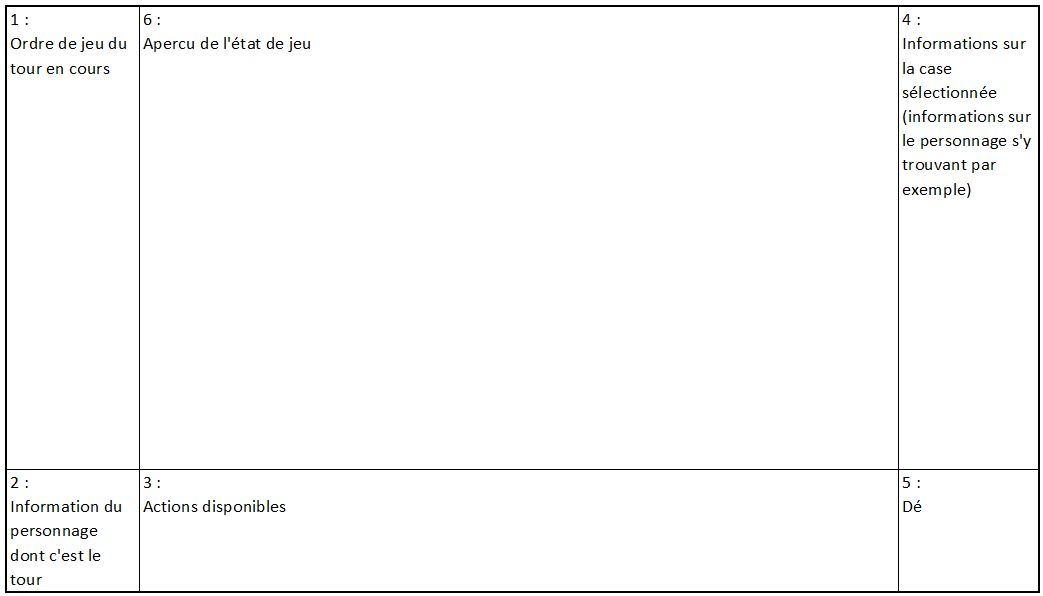
\includegraphics[scale=0.7, angle=0]{images/plan.png}
    \caption{Plan de l'affichage}
    \label{fig:plan}
\end{figure}

\begin{itemize}
    \item Case 1 : affichera le nom et l'ordre des entités en jeu (héros comme ennemis) et à terme pourrait aussi afficher le personnage en lui-même.
    \item Case 2 : affichera des informations de base (PV, PM, etc.) du personnage en train de jouer.
    \item Case 3 : nous permettra d'afficher les actions disponibles (attaquer, se déplacer...) et à terme nous pourrons afficher sur le terrain la portée de l'action sélectionnée. 
    \item Case 4 : nous permet d'afficher les informations sur la case sélectionnée, si elle est vide le menu sera vide mais si un personnage est sur cette case cela affichera les informations de celui-ci. A terme nous pourrions rajouter les informations sur un objet déposé ou n'afficher les informations que si le monstre a déjà été affronté etc.
    \item Case 5 : nous permettra d'afficher le résultat du dé après la réalisation d'une action.
    \item Case 6 : nous permettra d'afficher le terrain en lui-même et les personnages.
\end{itemize}

Il sera nécessaire de gérer le nombre d'éléments maximum affichage (pour les actions ou le terrain par exemple) pour éviter qu'une case ne dépasse sur une autre ou des conflits entre les menus et les sélections du joueur.

De plus il nous faudra gérer plusieurs mode différents : le mode de jeu que nous avons défini ici, le mode menu, le mode nouvelle partie, etc.

Pour l'exemple, nous générons un état avec trois entités (Diana, Charles et Elisabeth) avec chacun une position et quelques statistiques, ainsi que des actions supplémentaires et voilà un rendu provisoire de ce à quoi le menu jeu pourra ressembler dans ce cas :
\begin{figure}[hbt!]
    \centering
    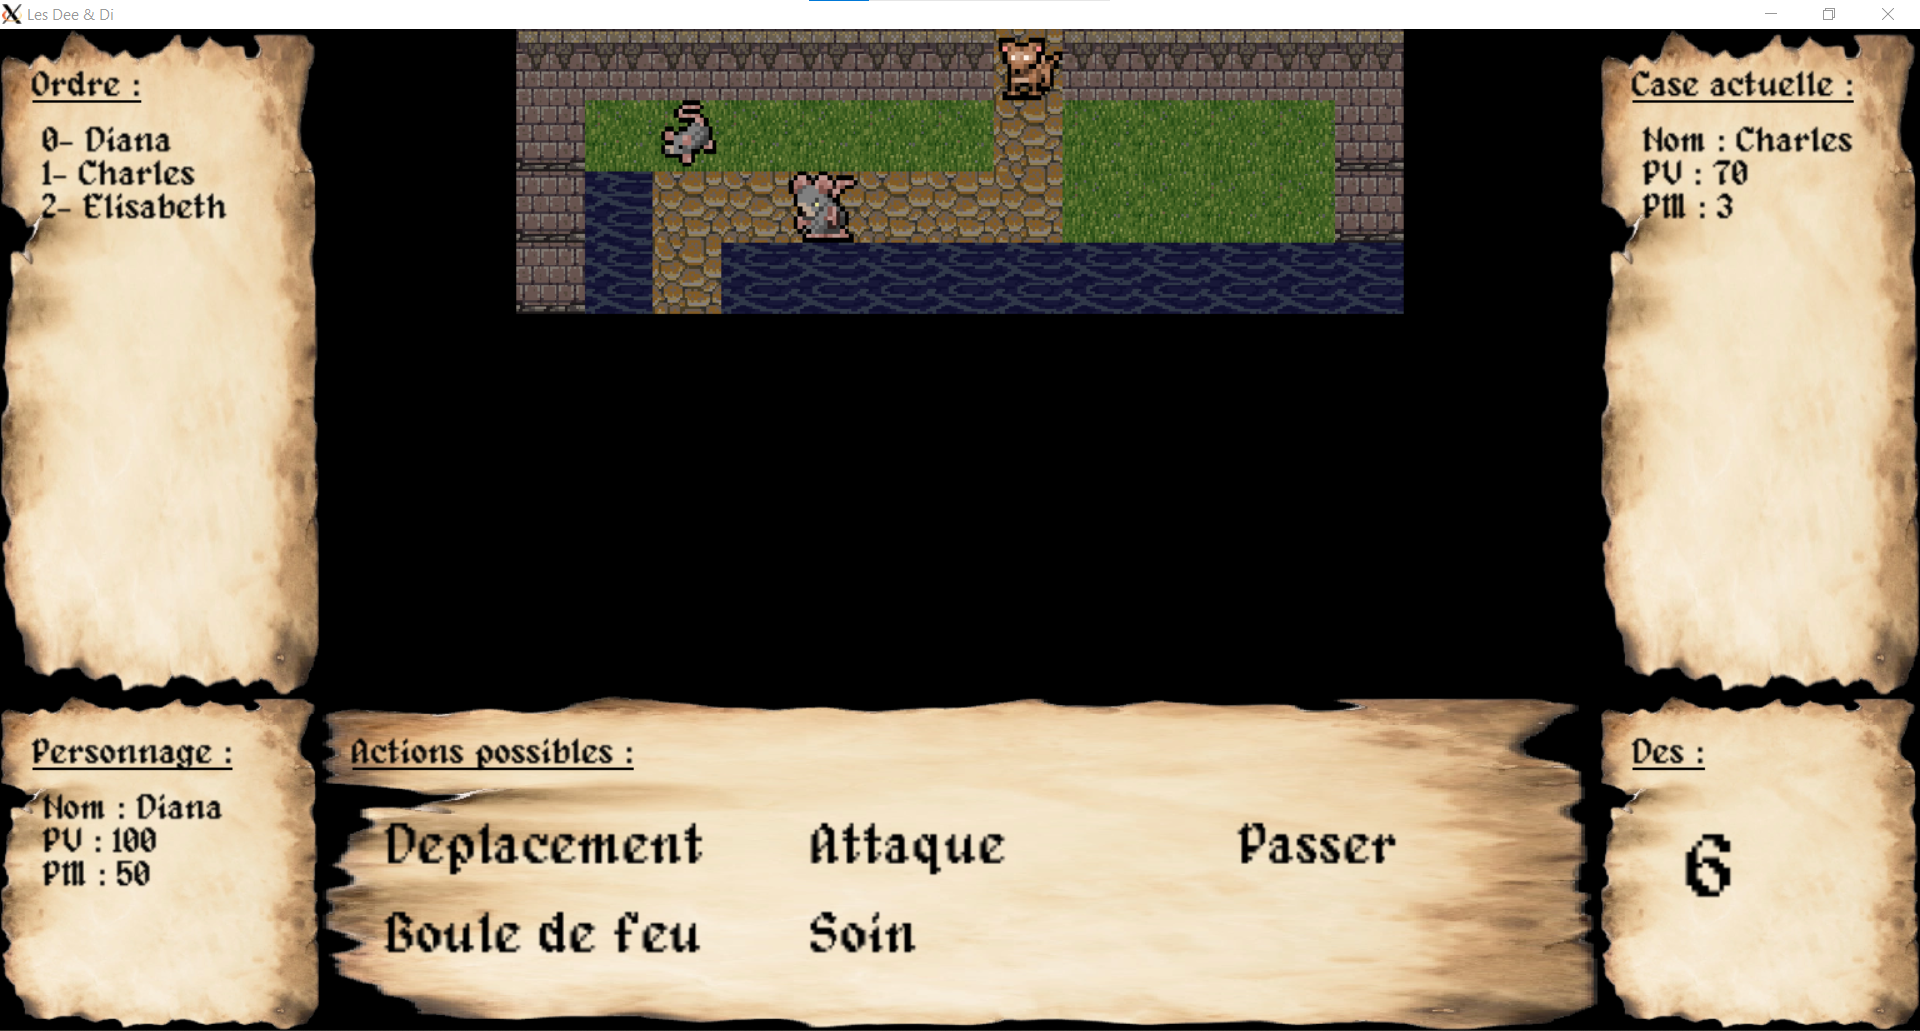
\includegraphics[width =.8\paperwidth, angle=0]{images/rendu.png}
    \caption{Rendu de l'affichage}
    \label{fig:rendu}
\end{figure}
\newpage

\subsection{Conception logiciel}

Pour la conception logiciel, nous avons décidé de fonctionner par couche, avec deux types de couches : les couches menus, qui afficherons majoritairement du texte avec un agencement précis, et les couches de terrain qui se chargerons d'afficher l'état du jeu donc le terrain en lui-même, les personnages et la portée de l'action sélectionnée. Nous avons donc deux classes qui héritent d'une classe couche globale qui nous permet de gérer plus facilement leur affichage.

L'organisation et l'affichage est géré par un objet Scene, qui va répertorier à la fois l'état de jeu, l'état du joueur, pour permettre l'affichage dans les couches. Ainsi les couches en elles-mêmes n'ont aucune information sur l'état de jeu et se contente d'afficher les informations issues de la scène. Pour permettre l'affiche, nous utilisons les classe sf::Transformable et sf::Drawable comme interface pour les couches.

Concernant l'affichage dynamique de l'état de jeu, nous avons une fenêtre qui reste affichée tant qu'elle n'est pas fermé et vérifie l'état de jeu toutes les seize millisecondes (60Hz), pour afficher l'état actuel. Plus tard, nous pourrons implémenter une fonction qui n'affiche l'état actuel qui si celui-ci a changé, réduisant ainsi les appels.

\begin{figure}[hbt!]
    \centering
    \includegraphics[width =.8\paperwidth, angle=0]{images/render.png}
    \caption{Diagramme de classe de render}
    \label{fig:render}
\end{figure}



%\begin{landscape}
%\begin{figure}[p]
%\includegraphics[width=0.9\paperheight]{render.pdf}
%\caption{\label{uml:render}Diagramme des classes de rendu.} 
%\end{figure}
%\end{landscape}

\clearpage
\section{Règles de changement d'états et moteur de jeu}

\subsection{Règles}
Nous allons commencer par des règles simples. Un personnage ne peut se déplacer que du nombre de cases indiqué par sa statistique de portée et ne peut attaquer ou utiliser une action supplémentaire qu'une seule fois par tour. Une fois ces actions effectuées, le joueur choisi quand laisser son tour se finir (lui laissant ainsi le loisir de lâcher un équipement par exemple). Concernant le déplacement, une entité peut se déplacer au maximum de sa statistique de déplacement sans traverser ni les murs ni les personnages et ne peut donc pas s'y arrêter. Il en va de même pour la portée des attaques ou des autres actions avec la statistique de portée. Les actions supplémentaires défensives soignent des Points de Vie (PV), dans la limite des PV maximum de l'entité (définis dans les statistiques de chaque entité.

\subsection{Conception logiciel}
Pour la conception logiciel, nous avons créé une classe Engine, qui stocke l'état actuel ainsi qu'un attribut json qui nous permettra à terme d'enregistrer les données du jeu. Cette classe Engine utilise des éléments de la classe Commande avec la méthode "addCommande". Cette dernière permet de vérifier si l'action lié à la commande est valide et si il l'est elle actualise l'état. De la classe abstraite Commande héritent trois classes : CommandeDeplacement, CommandeAttaque et CommandeActionSupplementaire. Elles permettent respectivement de créer une commande qui permet d'effectuer un déplacement, une attaque ou bien une action supplémentaire (comme un sort). Chacune de ses classes possède des méthodes handle (qui sont aussi virtuelle dans la classe Commande) qui permettent de vérifier les différentes règles liés à l'action.

%\begin{landscape}
%\begin{figure}[p]
%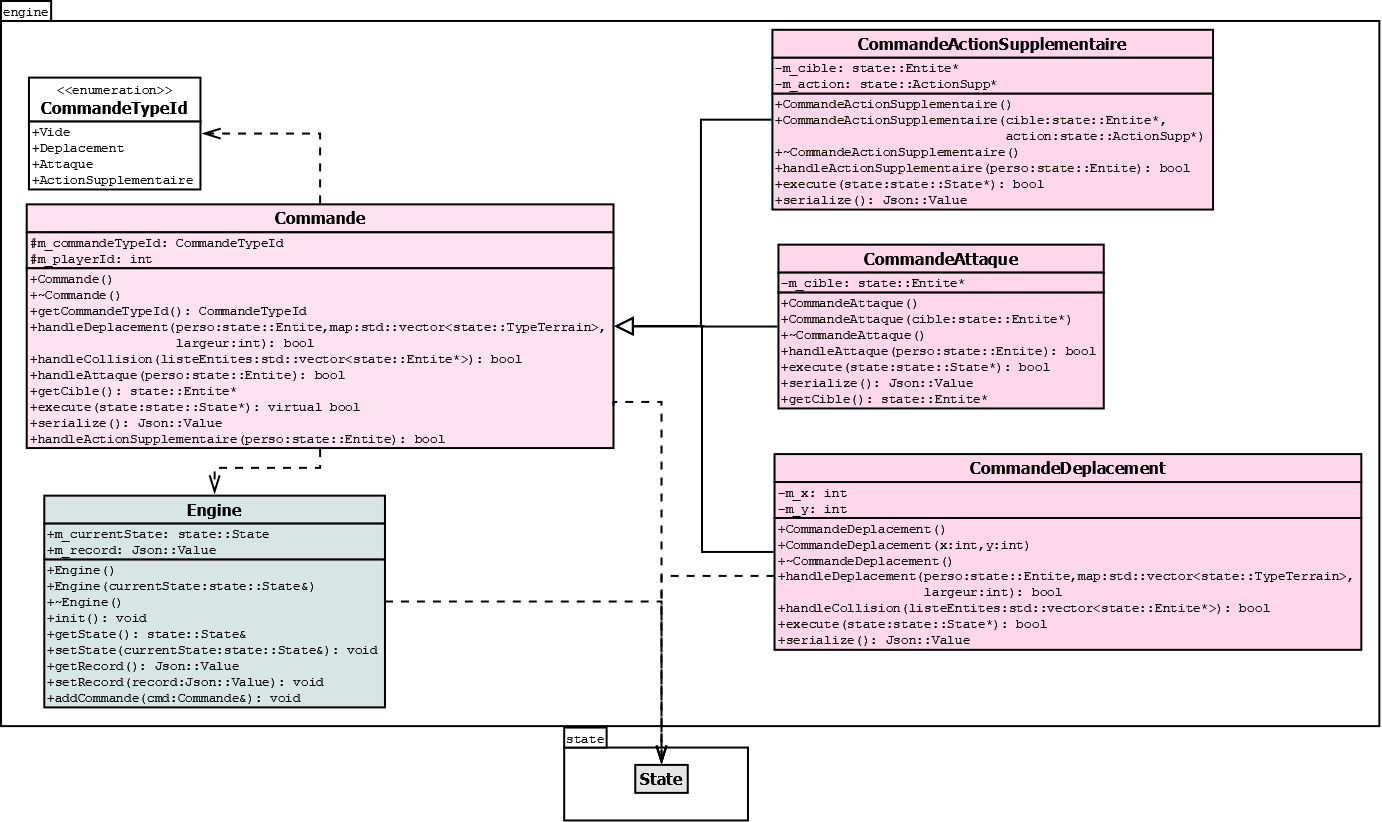
\includegraphics[width=0.9\paperheight]{engine.pdf}
%\caption{\label{uml:engine}Diagramme des classes de moteur de jeu.} 
%\end{figure}
%\end{landscape}

\clearpage
\section{Intelligence Artificielle}


\subsection{Stratégies}
L'intelligence artificielle aléatoire a accès aux différentes commandes du moteur de jeu. Lorsqu'elle agit, elle choisit une de ces commandes au hasard. Les paramètres associés sont aussi choisis de manière aléatoire, tels qu'ils donnent lieu à une commande valide.

L'intelligence artificielle peut déplacer l'entité dont c'est le tour sur une case du plateau accessible par cette entité. Cette case est choisie de façon aléatoire.

Elle peut aussi essayer d'attaquer une entité choisie au hasard. Si aucune entité n'est à portée, elle passe son tour.

\subsection{Conception logiciel}
Le diagramme des classes pour l'intelligence artificielle est présenté en Figure 9.

La classe AI donnera lieu à des classes héritées implémentant différentes intelligences artificielles plus ou moins poussées.

La classe RandomAI implémente une intelligence artificielle dont les actions sont dictées par l'aléatoire. Sa donnée membre m\_mt est un générateur de nombres aléatoires.

\begin{figure}[hbt!]
    \centering
    \includegraphics[width =.8\paperwidth, angle=0]{images/ai.png}
    \caption{Diagramme de classes d'ai}
    \label{fig:randomai}
\end{figure}

%\begin{landscape}
%\begin{figure}[p]
%\includegraphics[width=0.9\paperheight]{ai.pdf}
%\caption{\label{uml:ai}Diagramme des classes d'intelligence artificielle.} 
%\end{figure}
%\end{landscape}

\clearpage
\section{Modularisation}
\label{sec:module}

\subsection{Organisation des modules}


\subsection{Conception logiciel}


%
%\begin{landscape}
%\begin{figure}[p]
%\includegraphics[width=0.9\paperheight]{module.pdf}
%\caption{\label{uml:module}Diagramme des classes pour la modularisation.} 
%\end{figure}
%\end{landscape}

\end{document}
